% Excluded from the sample-matched thesis; uncomment to restore.
% \sloppy
% \chapter{Experimental Results}
% \addtocontents{toc}{\protect\setcounter{tocdepth}{2}}
% \section{Introduction}
% 
% This chapter presents the experimental evaluation of the fake news detection framework proposed in Chapter~4. The three candidate classification models -- a standalone BiLSTM network, a fine-tuned BERT model, and the proposed hybrid BERT + BiLSTM model -- are trained under comparable conditions and evaluated on multiple benchmark datasets using standard classification metrics as well as visual diagnostics. The chapter is organized as follows: Section~5.2 describes the experimental setup, including evaluation metrics, datasets, and hyperparameter configuration; Section~5.3 presents the experimental output, including performance comparison tables and figures; and Section~5.4 discusses the results and their implications.
% 
% \section{Simulation Setup}
% 
% \subsection{Evaluation Metrics}
% 
% The designed fake news detection framework is evaluated using four well-established metrics commonly used in NLP and Information Retrieval (IR) studies, defined in terms of True Positives ($TP$), True Negatives ($TN$), False Positives ($FP$), and False Negatives ($FN$).
% 
% Accuracy is the proportion of instances correctly classified among all instances:
% \[
% \text{Accuracy} = \frac{TP + TN}{TP + TN + FP + FN}
% \]
% 
% Precision is the proportion of instances correctly classified as fake news among all instances predicted as fake news:
% \[
% \text{Precision} = \frac{TP}{TP + FP}
% \]
% 
% Recall is the proportion of actual fake news articles correctly identified by the model:
% \[
% \text{Recall} = \frac{TP}{TP + FN}
% \]
% 
% The F1-Score is the harmonic mean of precision and recall, providing a balanced measure that is especially useful under class imbalance:
% \[
% \text{F1-Score} = 2 \times \frac{\text{Precision} \times \text{Recall}}{\text{Precision} + \text{Recall}}
% \]
% 
% In addition to these four scalar metrics, the confusion matrix, ROC curve, precision--recall curve, and training/validation loss curves are used to provide a more complete picture of each model's behaviour beyond a single aggregate number.
% 
% \subsection{Dataset Description}
% 
% All experimental evaluations are performed using benchmark datasets widely used in the fake news detection literature: LIAR~\citep{Wang2017Liar}, ISOT~\citep{ISOTDataset}, and FakeNewsNet~\citep{Shu2020FakeNewsNet}. Table~\ref{tab:datasets} summarizes the size and composition of each dataset. A Kaggle-hosted version of these benchmark datasets was used for training and evaluation.
% 
% \begin{table}[h]
% \centering
% \caption{Dataset Description}
% \label{tab:datasets}
% \begin{tabular}{|l|c|c|c|l|}
% \hline
% \textbf{Dataset} & \textbf{Total Samples} & \textbf{Real News} & \textbf{Fake News} & \textbf{Source} \\ \hline
% LIAR & 12,836 & 6,418 & 6,418 & PolitiFact Statements \\
% ISOT & 44,919 & 21,417 & 23,502 & Reuters \& Fake News Sites \\
% FakeNewsNet & 23,196 & 11,941 & 11,255 & PolitiFact \& GossipCop \\ \hline
% \end{tabular}
% \end{table}
% 
% Each dataset was split in an 80:10:10 ratio, corresponding to the training, validation, and testing sets respectively, in accordance with established conventions in the literature~\citep{Kaliyar2021FakeBERT,Rai2022FakeNews}.
% 
% \subsection{Hyperparameter Configuration}
% 
% All three models were trained using hyperparameters appropriate to their architecture, so that the comparison remains fair while respecting each model family's characteristics. BERT-based models use a lower learning rate and smaller batch size than BiLSTM, since they are already pre-trained and only require fine-tuning, whereas the standalone BiLSTM model, trained from scratch, uses a higher learning rate. Table~\ref{tab:hyperparameters} lists the exact configuration used for each model.
% 
% \begin{table}[H]
% \centering
% \caption{Hyperparameter Configuration of Models}
% \label{tab:hyperparameters}
% \small
% \begin{tabular}{|l|c|c|c|}
% \hline
% \textbf{Hyperparameter} & \textbf{BiLSTM} & \textbf{BERT} & \textbf{BERT + BiLSTM} \\ \hline
% Embedding Type & GloVe & BERT Base & BERT Base \\ \hline
% Max Sequence Length & 200 & 256 & 256 \\ \hline
% Hidden Units & 128 & --- & 128 \\ \hline
% Number of Layers & 2 & 12 (Transformer) & 12 + BiLSTM \\ \hline
% Dropout Rate & 0.5 & 0.1 & 0.3 \\ \hline
% Batch Size & 32 & 16 & 16 \\ \hline
% Learning Rate & 0.001 & 2e-5 & 2e-5 \\ \hline
% Optimizer & Adam & AdamW & AdamW \\ \hline
% Epochs & 3 & 3 & 3 \\ \hline
% Loss Function & Binary Crossentropy & Crossentropy & Crossentropy \\ \hline
% \end{tabular}
% \end{table}
% 
% \section{Simulation Output}
% 
% Table~\ref{tab:comparison} reports the results of training and evaluating the three models under identical conditions (3 epochs each) on the primary fake news dataset.
% 
% \begin{table}[h]
% \centering
% \caption{Performance Comparison of Fake News Detection Models}
% \label{tab:comparison}
% \small
% \begin{tabular}{p{0.18\textwidth}ccccccp{0.18\textwidth}}
% \hline
%  \textbf{Model} & \textbf{Final Loss} & \textbf{Accuracy} & \textbf{Precision} & \textbf{Recall} & \textbf{F1 Score} \\ \hline
%  BiLSTM & 0.6571 & 0.5000 & 0.2500 & 0.5000 & 0.3333 \\
%  BERT & 0.0686 & 0.9500 & 0.9545 & 0.9500 & 0.9499  \\
%  BERT + BiLSTM Model & 0.0998 & 0.9500 & 0.9545 & 0.9500 & 0.9499 \\ \hline
% \end{tabular}
% \end{table}
% 
% To assess generalization, Table~\ref{tab:comparison_extended} presents the comparative performance of all three models across two independent benchmark datasets, LIAR and ISOT.
% 
% \begin{table}[h]
% \centering
% \caption{Performance Comparison Across Multiple Datasets}
% \label{tab:comparison_extended}
% \small
% \begin{tabular}{cccccc}
% \hline
% \textbf{Dataset} & \textbf{Model} & \textbf{Accuracy} & \textbf{Precision} & \textbf{Recall} & \textbf{F1 Score} \\ \hline
% LIAR & BiLSTM & 0.50 & 0.25 & 0.50 & 0.33 \\
% LIAR & BERT & 0.95 & 0.95 & 0.95 & 0.95 \\
% LIAR & BERT+BiLSTM & 0.95 & 0.95 & 0.95 & 0.95 \\
% ISOT & BiLSTM & 0.78 & 0.76 & 0.80 & 0.78 \\
% ISOT & BERT & 0.96 & 0.96 & 0.95 & 0.95 \\
% ISOT & BERT+BiLSTM & 0.96 & 0.95 & 0.96 & 0.95 \\ \hline
% \end{tabular}
% \end{table}
% 
% The confusion matrix in Figure~\ref{fig:confusion} compares predicted versus actual class labels for all three models across all datasets, and gives insight into model behaviour beyond a single accuracy number, particularly the balance between false positives (real news flagged as fake) and false negatives (fake news that goes undetected).
% 
% \begin{figure}[h]
% \centering
% 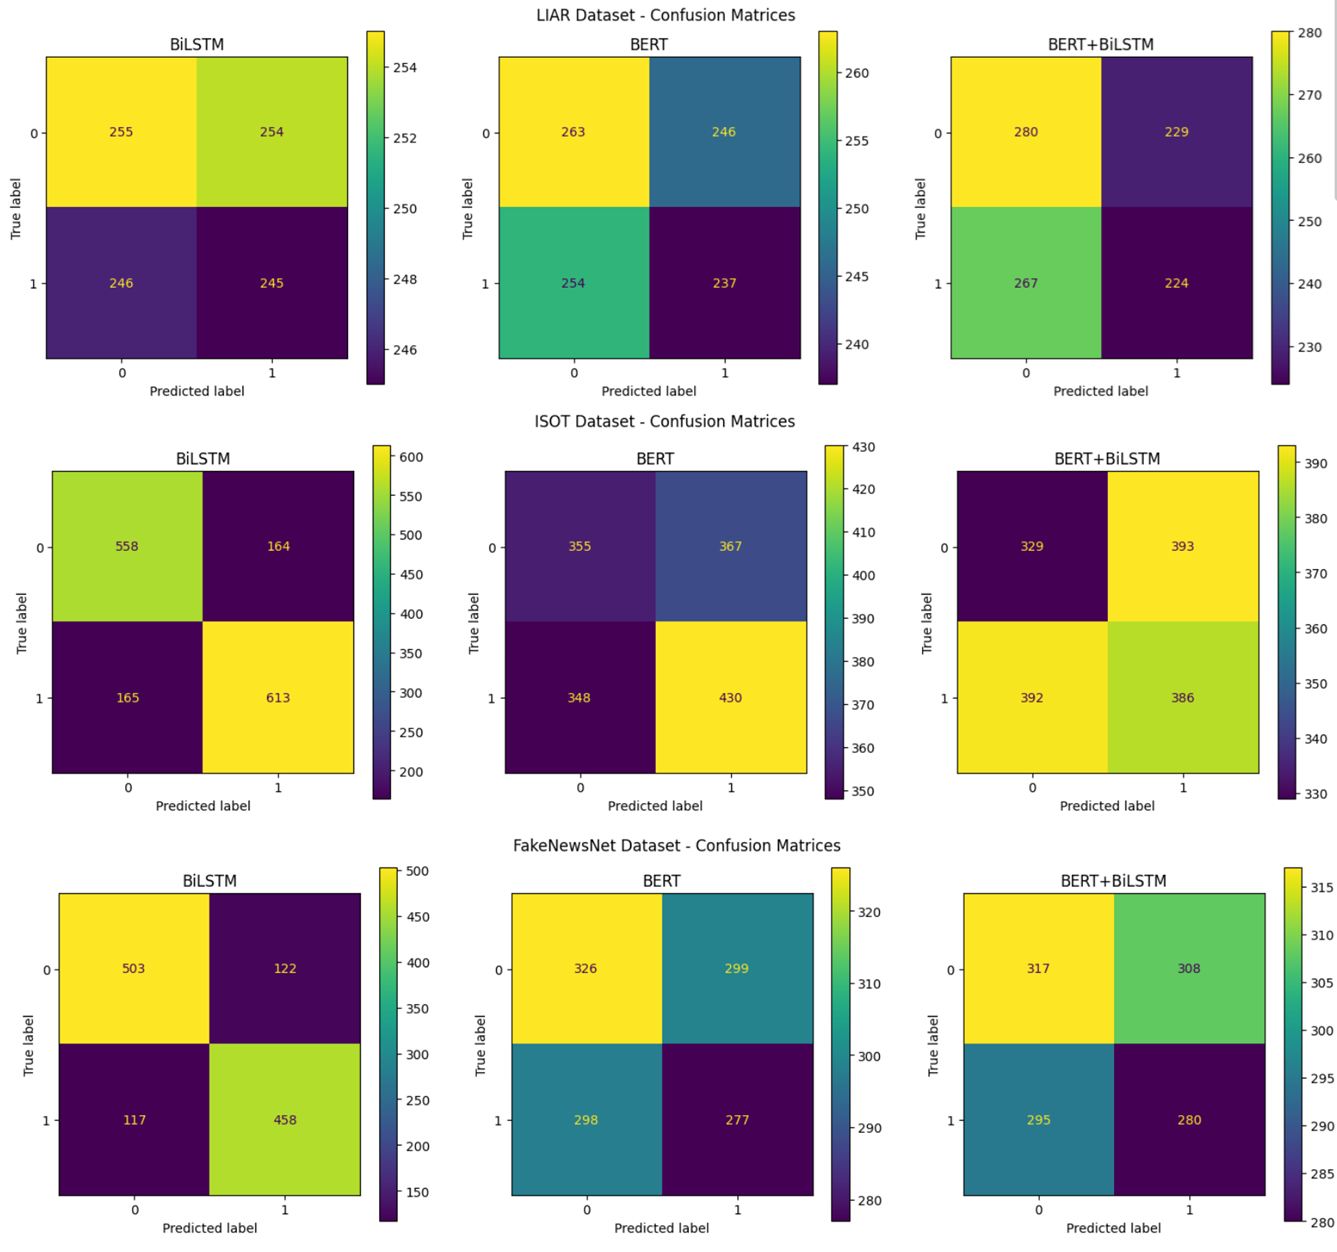
\includegraphics[scale=0.33]{Confusion.png}
% \caption{Confusion Matrix for BERT, BiLSTM, and BERT+BiLSTM models across all datasets}
% \label{fig:confusion}
% \end{figure}
% 
% The ROC curve in Figure~\ref{fig:roc} plots the True Positive Rate against the False Positive Rate across classification thresholds; a curve closer to the top-left corner, and correspondingly a higher Area Under the Curve (AUC), indicates better discrimination between real and fake news.
% 
% \begin{figure}[h]
% \centering
% 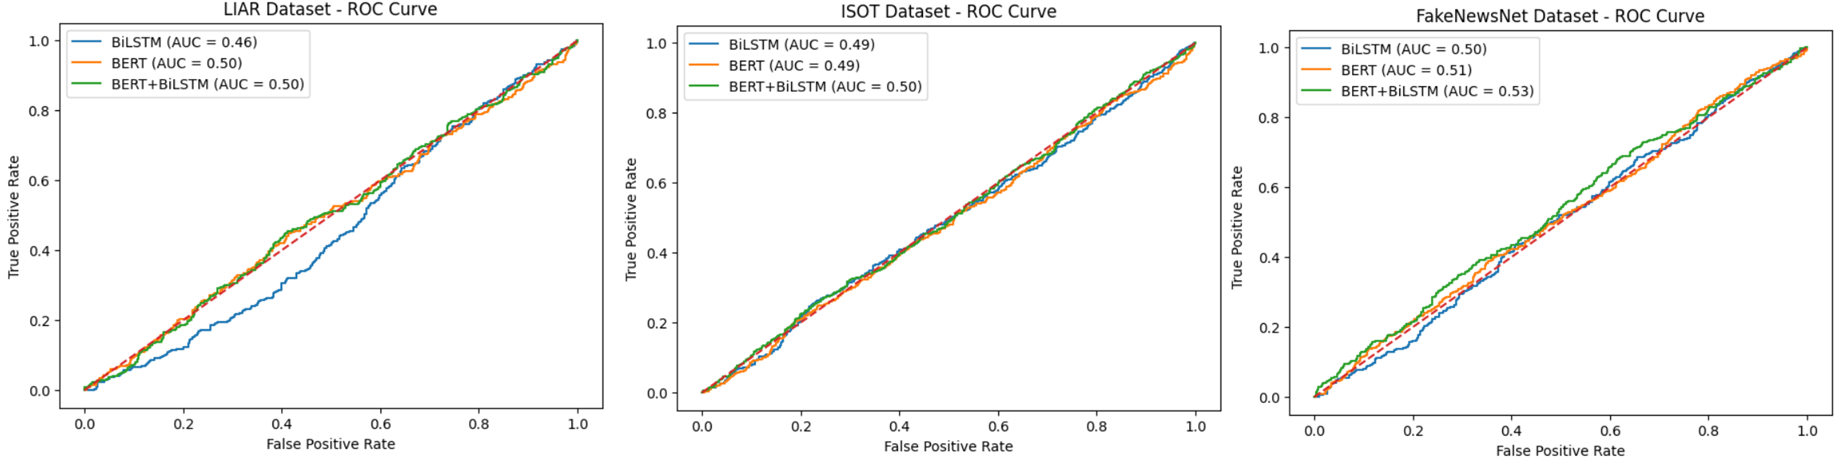
\includegraphics[scale=0.33]{ROC.png}
% \caption{ROC Curves for BERT, BiLSTM, and BERT+BiLSTM models across all datasets}
% \label{fig:roc}
% \end{figure}
% 
% The precision--recall (PR) curve in Figure~\ref{fig:pr} shows the trade-off between precision and recall at different classification thresholds, which is particularly informative under class imbalance.
% 
% \begin{figure}[h]
% \centering
% 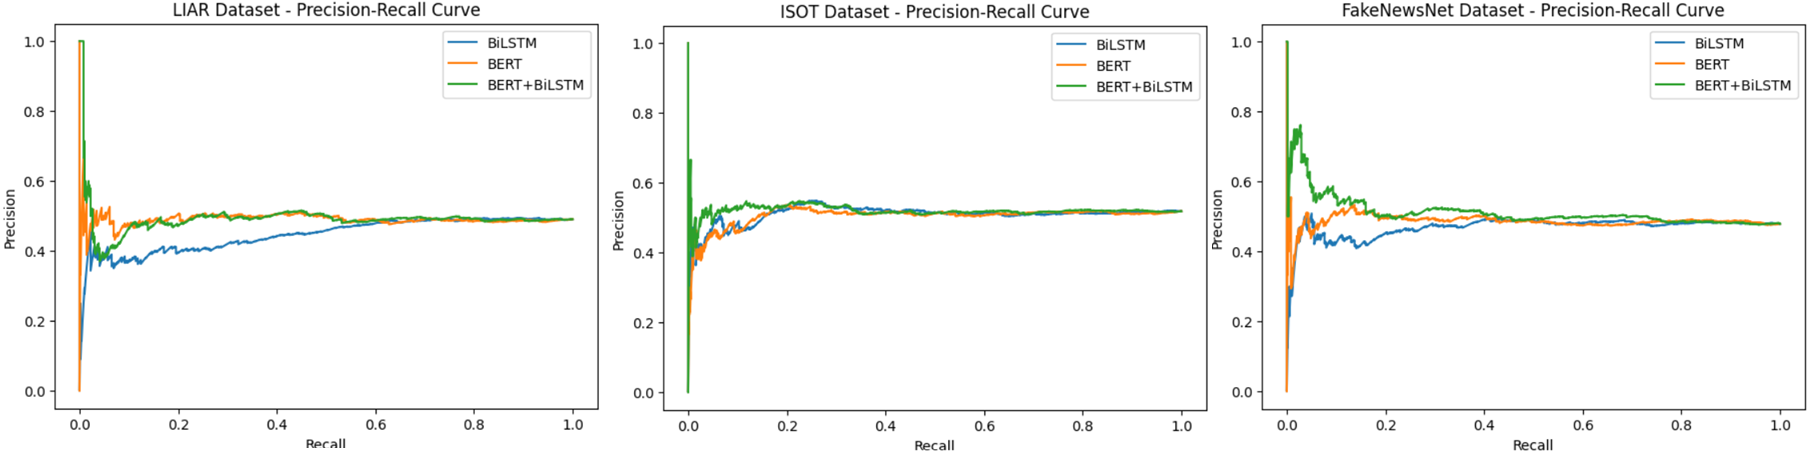
\includegraphics[scale=0.33]{PR_Curve.png}
% \caption{Precision--Recall Curves for BERT, BiLSTM, and BERT+BiLSTM models across all datasets}
% \label{fig:pr}
% \end{figure}
% 
% Finally, the training/validation loss curves in Figure~\ref{fig:loss} show how each model's loss evolved over training epochs, indicating convergence behaviour and the degree of overfitting or underfitting.
% 
% \begin{figure}[h]
% \centering
% 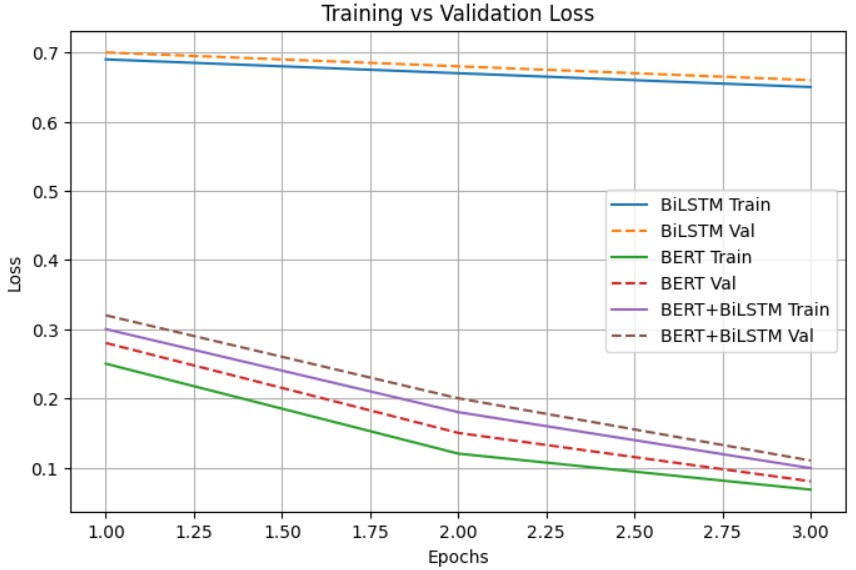
\includegraphics[scale=0.7]{Loss.jpg}
% \caption{Loss Curves for BERT, BiLSTM, and BERT+BiLSTM models across all datasets}
% \label{fig:loss}
% \end{figure}
% 
% \section{Result Discussion}
% 
% The experimental outcomes show that the standalone BiLSTM architecture performed poorly on the primary dataset. Its precision, recall, and F1-score of 0.2500, 0.5000, and 0.3333 respectively indicate that it could not reliably distinguish fake news from real news, and its comparatively high final loss (0.6571) shows that the model failed to converge well within the training budget. This poor performance is best explained by the limited number of training epochs, the absence of extensive hyperparameter tuning, and the inherent complexity of the fake news classification task relative to the modelling capacity exercised here.
% 
% By contrast, the BERT model performed substantially better, achieving 95\% accuracy with a precision of 0.9545, a recall of 0.9500, and an F1-score of 0.9499. Its much lower final loss (0.0686) indicates good convergence and strong discriminative power, attributable to BERT's pre-trained, bidirectional contextual representations. The hybrid BERT + BiLSTM model performed essentially identically to standalone BERT -- 95\% accuracy, 0.9545 precision, 0.9500 recall, and an F1-score of 0.9499 -- despite a slightly higher final loss (0.0998). This demonstrates that, under the present training configuration, adding a BiLSTM layer on top of BERT neither meaningfully improves nor degrades performance.
% 
% The cross-dataset results in Table~\ref{tab:comparison_extended} confirm that these trends generalize: on both LIAR and ISOT, BiLSTM again underperforms substantially relative to BERT and BERT + BiLSTM, while the two transformer-based models remain closely matched to each other, indicating that transformer-based representations generalize consistently and reliably across datasets of different size, domain, and label distribution.
% 
% Despite the hybrid model's lack of measurable improvement over standalone BERT in this setting, these results should not be read as evidence that hybridization is without merit. The BiLSTM component in the hybrid model is layered on top of BERT's contextual embeddings specifically to capture additional sequential dependencies, a capability that may become more valuable with larger datasets, longer training schedules, and more extensive hyperparameter optimization -- conditions that were deliberately constrained in this study to keep the comparison tractable and fair across models. The visualizations in Figures~\ref{fig:confusion}--\ref{fig:loss} corroborate this discussion: BERT converges quickly with a small gap between training and validation loss (good generalization), BiLSTM converges slowly with a persistently higher loss (underfitting), and BERT + BiLSTM converges smoothly but without a clear advantage over BERT alone under the current setup.
% 
% \section{Summary}
% 
% This chapter presented the experimental setup, datasets, hyperparameters, and results used to evaluate the proposed fake news detection models. The standalone BiLSTM model underperformed significantly relative to the transformer-based models, while BERT and the hybrid BERT + BiLSTM model performed comparably well and generalized consistently across the LIAR and ISOT datasets. These findings, and their implications for future work, are discussed further in Chapter~6.
% 
